% vim:set et sw=2 ts=4 tw=72:
\chapter{Introduction}

Version control records the changes being made to the files of a
project, enabling users to view previous versions of the files, view the
individual changes made, and restore the files back to a previous state
if necessary. The version control system also maintains a log of who
made changes and when those changes were made. By storing this
information, the version control system stores the history of the
project. Presented in the right way, there are many opportunities to use
this information to help users understand the architecture of the
software system, who is making changes, and which files are being
changed the most. While version control can be used in any context where
file history is desirable, version control is usually used in the
software development process.

Git is the \define{version control system}{VCS} designed for and used by
the Linux kernel project. In order to handle the number of people
contributing to the kernel from different countries, git was designed to
be distributed. Unlike in centralized repositories, where users must
re-synchronize with the server, a distributed version control system
provides each user with a full first-class repository. This allows the
user to have additional flexibility, and means that a user has to
synchronize less often. Furthermore, each user has a copy of the entire
repository, which means that they have access to all of the branches and
commits in the repository. This gives users the ability to change the
structure of the repository and make changes that would not work in a
centralized repository. To make it more useful to the Linux project, git
was designed to allow easy branching. Branches allow users to work on a
logically separate part of the repository, then the changes into the
repository once the feature is finished or the bug is fixed. This lets
users work for longer without needing to synchronize with the rest of
the project as often. To support these requirements, git uses a directed
acyclic graph to represent the repository. The nodes of the graph
represent the commits, containing the actual changes being made, along
with metadata about who is making the changes, when the changes were
made, and the parent nodes of the commit.

Visualizations of the graph are used to answer questions about the
development of the software including what changes are being made into
various branches, how the changes to the code are grouped, and who is
working with whom, among others. Maintainers use the visualizations to
understand what changes are being made to the current version of the
software in order to apply the necessary fixes to older versions of the
software to keep them secure and performing correctly. This requires
understanding how a commit is integrated into the repository, and other
commits that are merged with that commit. In large, active, software
repositories this task is not trivial. The graph can be large and
complicated, making the visualizations difficult to understand.

This \paper{} makes four contributions. First, a new tree-based model,
called the \mt{}, constructed from the underlying graph of the
repository. Compared to the graph, trees are relatively easy to
visualize, and there are many visualization metaphors that take
advantage of different properties of the trees. There are visualizations
designed for both short wide trees, as in the case of file systems, and
tall narrow trees. Furthermore, trees have fewer edges and relatively
strict properties, meaning that the visualizations are simpler. Second,
visualizations that take advantage of the \mt{} model. Third, an
implementation of the visualizations in a tool, called \tool{}. Finally,
an evaluation of the tool to determine whether visualizing the
repository using the model is useful. This \paper{} specifically studies
the Linux repository. The Linux repository is large and complex, with
more than 1000 contributors making changes every release. Details about
the repository are provides in Section~\ref{sec:linux}.

The central thesis of the paper is finding a means of visualizing a
repository that is as large and complex as the Linux repository in a
meaningful way that gives insight into how commits are integrated.

\begin{textbox}
  \textbf{Thesis:} How do we effectively visualize the graph of the
  Linux repository in a way that gives insight into how commits are
  integrated?
\end{textbox}

\section{Related Work}\label{sec:related_work}

The Version Control System tracks the development of a software project,
recording each change as it happens. By tracking the changes, the VCS
contains an entire story of the software, rich with information about
who the authors are, what files are being modified, what where changes
are being made. This makes the VCS vital in providing information about
how a software project is being developed and how the software is
structured. In order to use the information stored in the VCS, users
must be able to gain a clear understanding and summarization of the
changes being made, and how they interact with the rest of the source
code. While there has been extensive research on visualizing software
repositories, previous work does not focus on how commits and merges are
structures in the repository graph, and in extension, how commits are
integrated into a repository. The literature on repository visualization
and summarization can be broken down into three academic subcategories;
communication\cite{Cubranic2005,Begel2010}, aspect-oriented
visualization\cite{Ambros2005,Burch2005,Ambros2009}, and organic
visualizations\cite{ogawa09,Caudwell2010}. A fourth industrial category
exists, including tools like GitKraken and SourceTree. The goal of the
industrial tools is not to extract or synthesize new information from
the repository, but to act as a user-friendly client on top of what git
already provides.

Many tools focus on addressing the issue in communication between
developers in inter-team collaborative work. Hipikat\cite{Cubranic2005}
investigates communication between developers, focusing on assisting
with the integration of new developers into a project though
communication, providing the new developer with searchable artifacts of
the changes being made, and where to find them. The artifacts may
include files or bug information, shown in Figure~\ref{fig:hipikat}.
Codebook\cite{Begel2010} also focuses on communication, but where
Hipikat focuses on assisting new developers find artifacts, Codebook
assists developers with finding who was responsible for creating the
artifact. Codebook uses a data-mining technique to determine the
developer of a piece of code, the program manager who wrote the
specification for the code, and the program managers and developers on
the team who were working together. A screenshot of Hoozizat, an
implementation of codebook, is shown in Figure~\ref{fig:codebook}.
Hoozizat and Hipikat use the version control as the archive of artifacts
that are being queried. Neither tool is designed with the goal of
providing information on the topological structure of a source code
repository, nor are these tools designed for visualization purposes, but
they do draw information from the contents of the version control
system.

\begin{figure}[htpb]
  \centering
  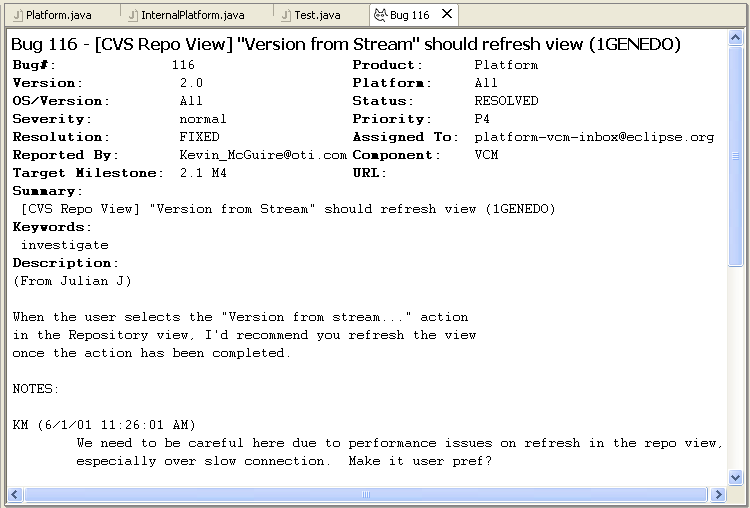
\includegraphics[width=0.9\linewidth]{Figures/introduction/hipikat_bug.png}
  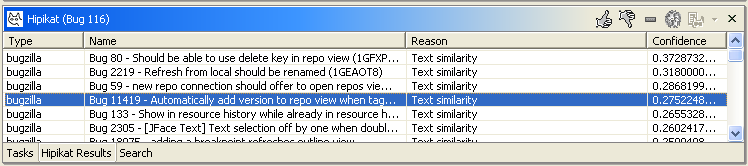
\includegraphics[width=0.9\linewidth]{Figures/introduction/hipikat.png}
  \caption{View of Hipikat, listing bugs that are similar to the one
  being viewed}
  \label{fig:hipikat}
\end{figure}

\begin{figure}[htpb]
  \centering
  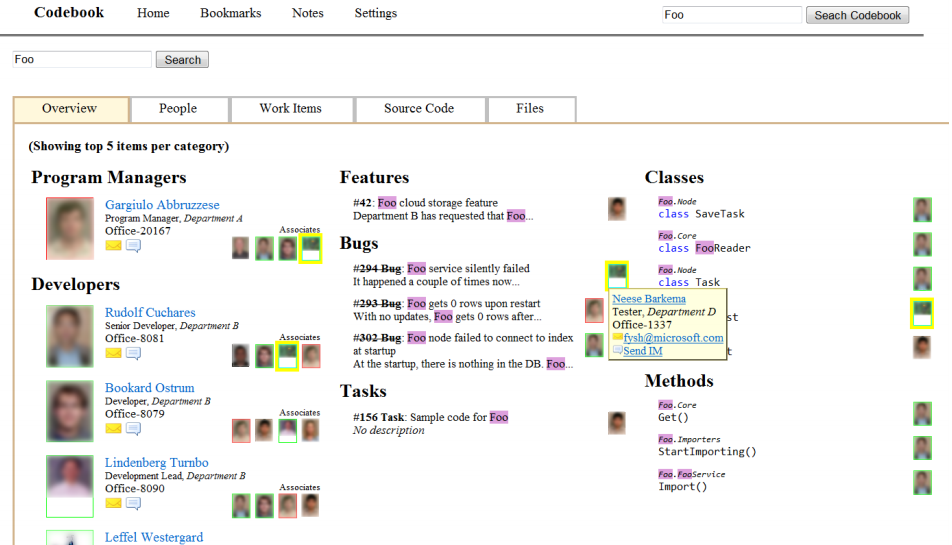
\includegraphics[width=0.8\linewidth]{Figures/introduction/codebook.png}
  \caption{A screenshot of the search results on Hoozizat, an
    implementation of codebook.}
  \label{fig:codebook}
\end{figure}

Most visualization systems provide information about a certain aspect of
the contents in the repository. The goal being Fractal
Figures\cite{Ambros2005} is to show the division of work between
contributors. The project is represented as a square. The square is then
subdivided based on the proportion that a given contributor contributed
to the project, shown in Figure~\ref{fig:fractal_figures}. The
visualization makes it easy to see where work is evenly divided versus
the projects where a single contributor is doing most of the work.

\begin{figure}[htpb]
  \centering
  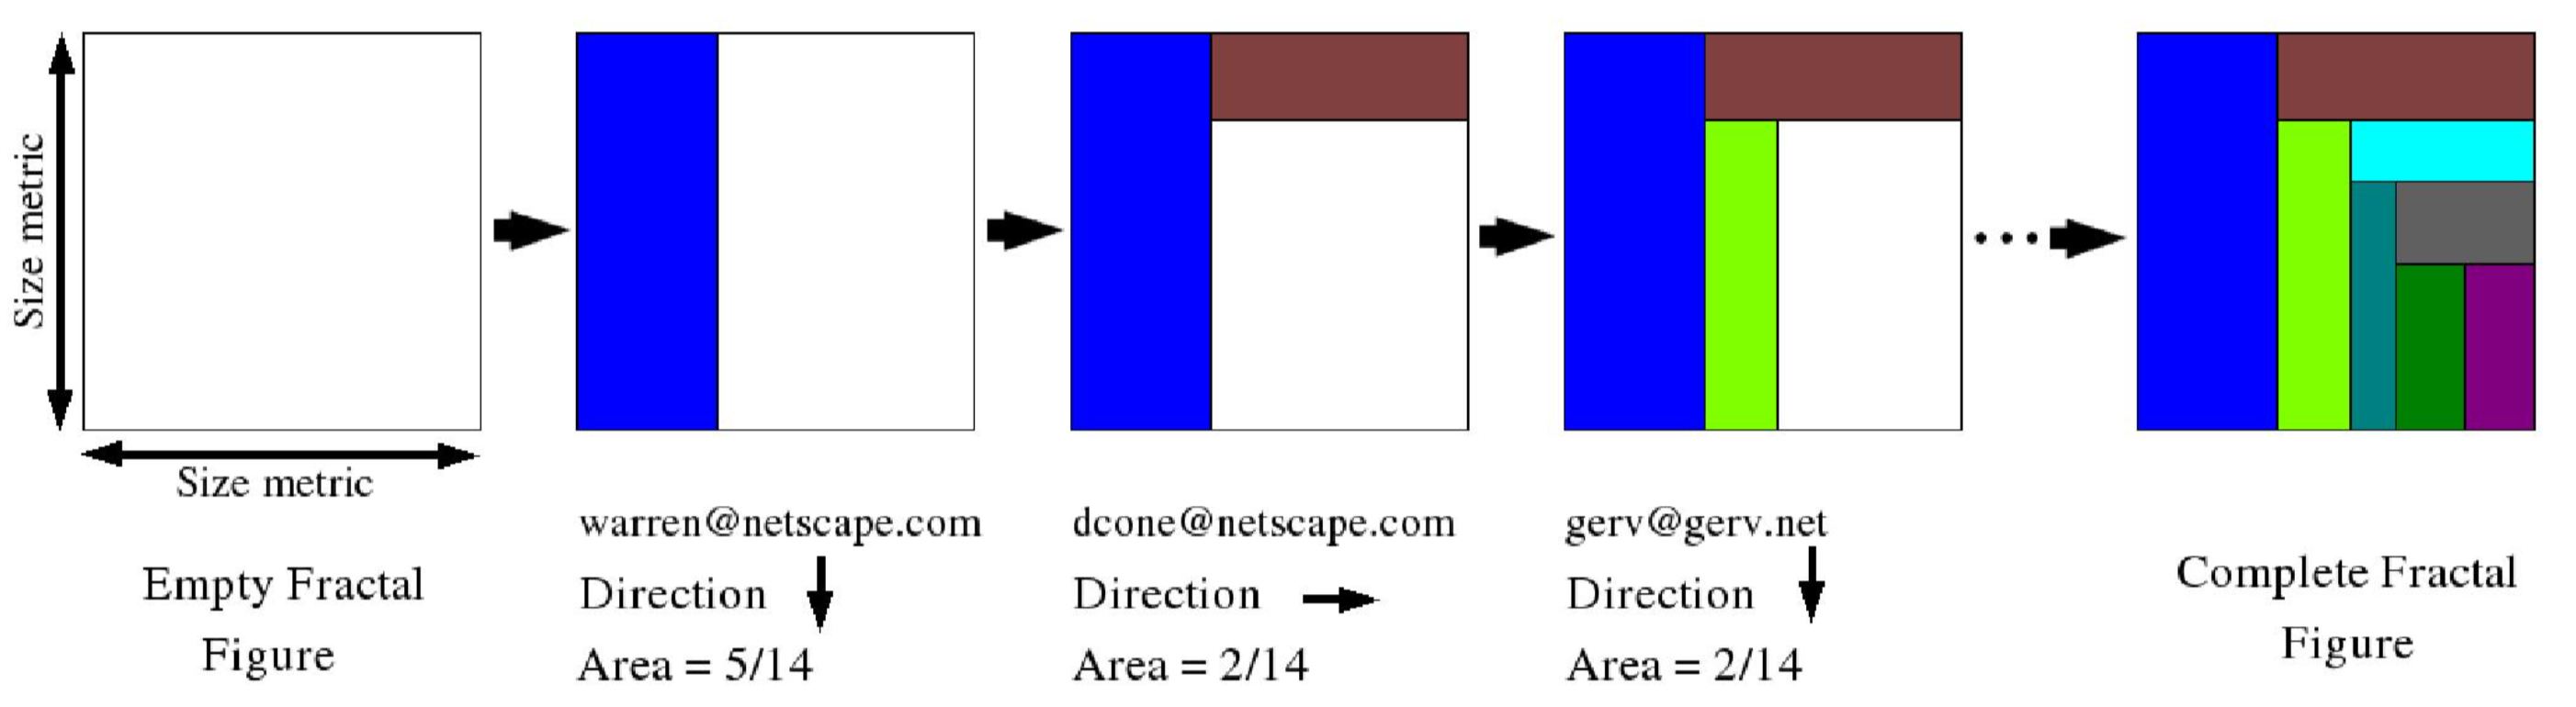
\includegraphics[width=0.8\linewidth]{Figures/introduction/fractal_figures.png}
  \caption{Construction of Fractal Figures}
  \label{fig:fractal_figures}
\end{figure}

EPOSee\cite{Burch2005} and Evolution Radar\cite{Ambros2009} use the
information from the version control to determine which files are edited
together. The tools from these papers are designed to help a user
identify the degree to which two files are coupled. Two files are
edited and committed together frequently are said to be more tightly
coupled. This makes it possible to determine when two classes are
semantically related. The evolution radar shown in
Figure~\ref{fig:evolution_radar} places points on a circle based on the
name and coupled they are. The files are arranged around the circle
based on the file name, including the full file path. This has the
effect of grouping files that are from the same directory. The distance
from the center of the circle is dependent on how tightly coupled the
file is to the file be analyzed. A more tightly-coupled file will be
positioned more closely to the center of the circle.

\begin{figure}[htpb]
  \centering
  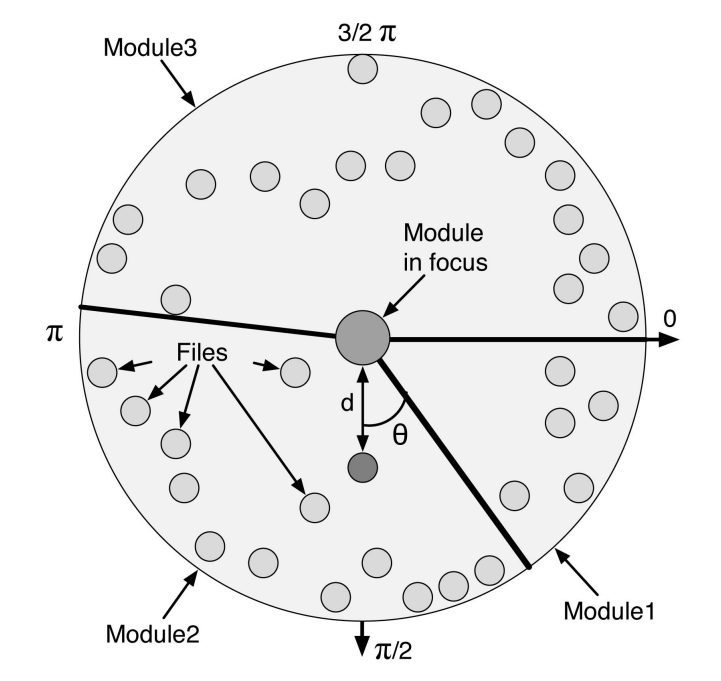
\includegraphics[width=0.8\linewidth]{Figures/introduction/evo_radar.png}
  \caption{Evolution Radar visualization}
  \label{fig:evolution_radar}
\end{figure}

Hoozizat, Hipikat, Fractal Figures, EPOSee, and Evolution Radar all
extract data from CVS repositories. Our goal is to provide information
about git repositories. Fewer tools are available for generating
visualizations and summaries of git repositories, potentially due to the
DAG model used as the internal structure of git repositories.

Organic visualizations show patterns in cooperation and communication
that arise within a software project organically. Heller et
al.\cite{Heller2011} plots communication on a map. This visualization
shows communication and cooperation patterns that arise, and how they
cross country boundaries, within a software project.
Gource\cite{Caudwell2010}, shown in Figure~\ref{fig:gource_view}, shows
which files contributors are working on. Using this, it is possible to
draw conclusion about which parts of a project a given contributor is
working on and the group of contributors working on a given area. Gource
uses a graph metaphor structure to represent the file structure of a
repository. Files in the same directory cluster together to form a node.
Edges between the directory clusters represent which directory contains
another, although there is no way to determine the direction of the
relationship. User avatars move around the graph emitting different
beams of colored light depending on the change being made to the file.
Greed indicates the creation of a new file, yellow indicates a
modification, and red indicates the deletion of a file. The
visualization is animated to show how a project grows over time.
Codeswarm\cite{ogawa09}, shown in Figure~\ref{fig:codeswarm}, is similar
to Gource, using an organic timelapse approach to visualizing the events
in the repository. Unlike Gource, which constructs a graph from the
directory structure of project, Codeswarm does not have a graph
structure. Developers are the center of the visualizations. When a
developer makes a change to a file, the file lights up and flies toward
the developer. As a developer makes more changes, the files that the
developer is modifying will form a ring around the developer. If
multiple developers are modifying a file, the developer nodes are drawn
together.

\begin{figure}[htpb]
  \centering
  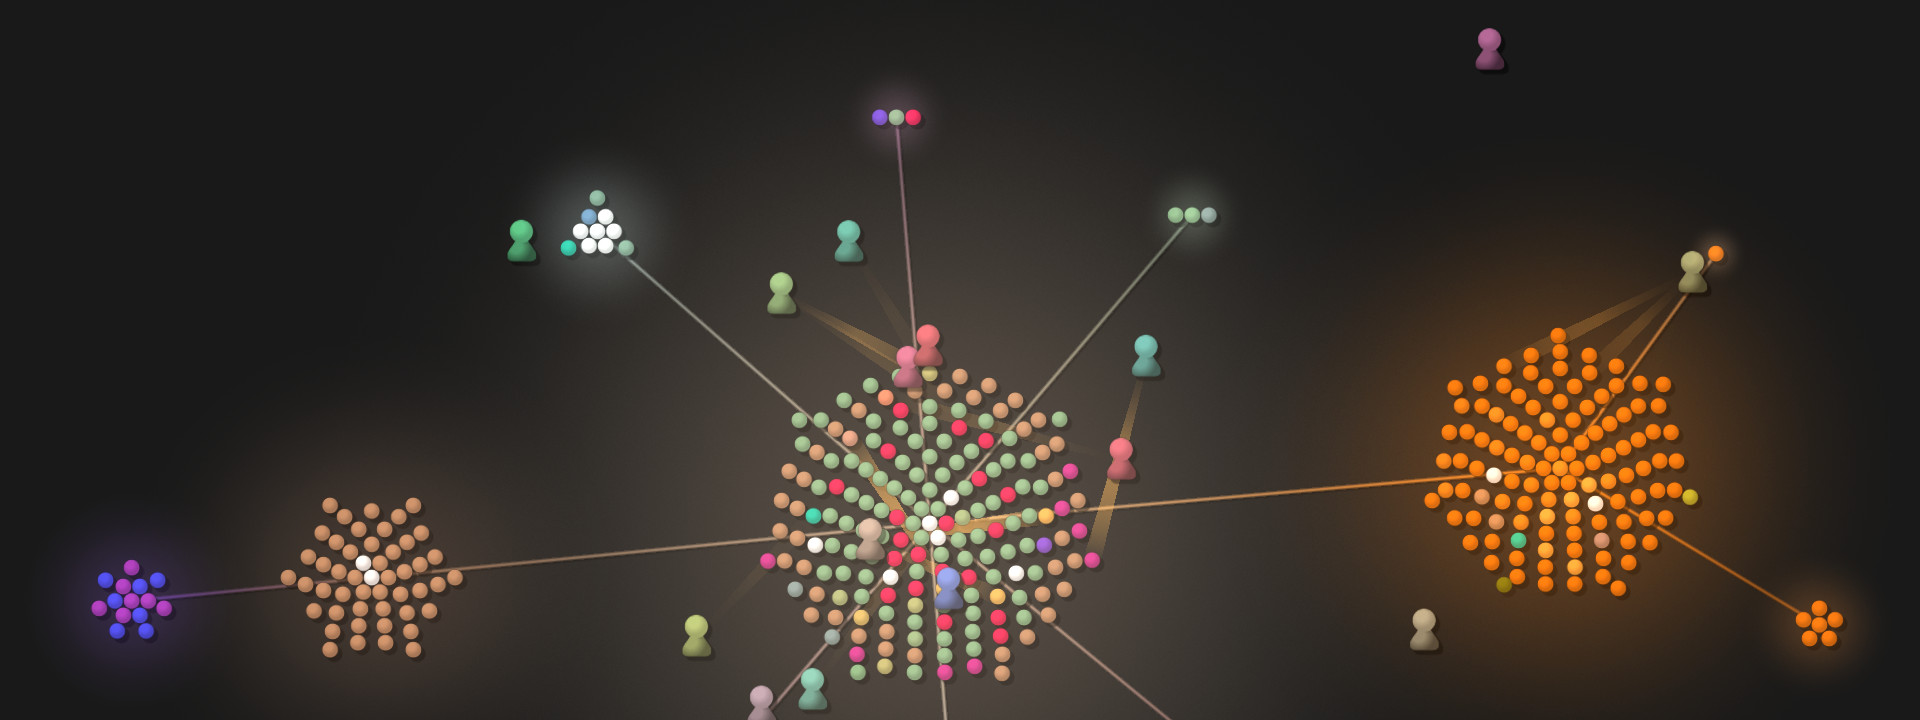
\includegraphics[width=0.8\linewidth]{./Figures/introduction/gource-linux.jpg}
  \caption{View of Gource file graph with users operating on a
    repository}
  \label{fig:gource_view}
\end{figure}

\begin{figure}[htpb]
  \centering
  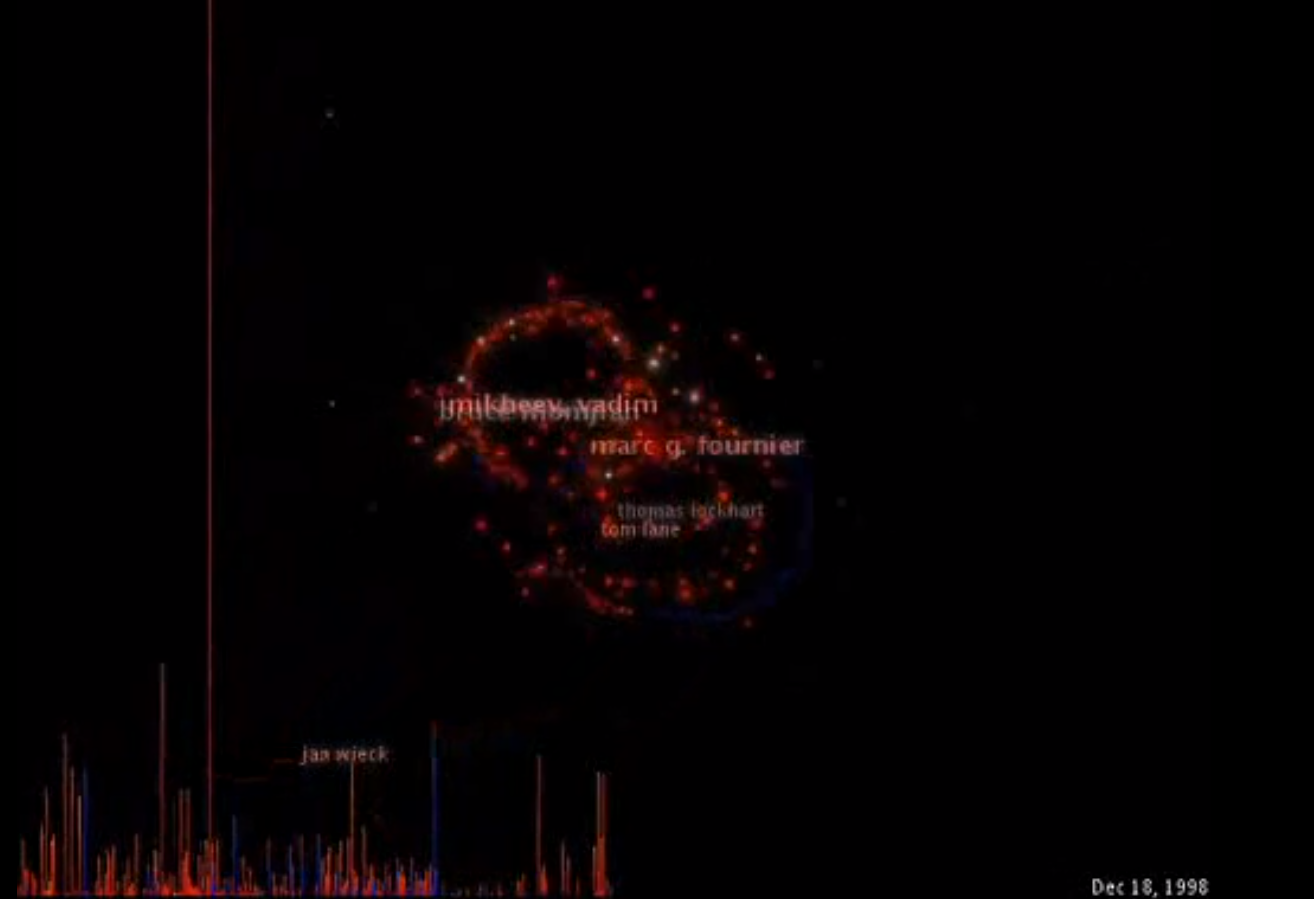
\includegraphics[width=0.8\linewidth]{Figures/introduction/codeswarm.png}
  \caption{View of the Postgresql repository in Codeswarm}
  \label{fig:codeswarm}
\end{figure}

There are many non-academic tools that are designed as an interface to
git. While not all of these programs provide visualizations, those that
do use a visual metaphor of the DAG to show topological information
about the repository. While they ultimately show the same information,
the topology of the repository, the organization of that information is
different.

GitKraken, shown in Figure~\ref{fig:gitkraken_main},  is a popular
commercially written git interface that aims to be efficient, elegant,
and reliable, according to the official website. On visual inspection,
it appears to satisfy these goals. Overall, the interface is clean, most
actions that are possible with the git command line are available in the
graphical interface. Overall, the tool is clean and garners online
approval from users. The graph itself, shown in the center of the main
view provides users with the same information as the graph visualization
in gitk and the git command line, though it may be visually more
appealing.

\begin{figure}[htpb]
  \centering
  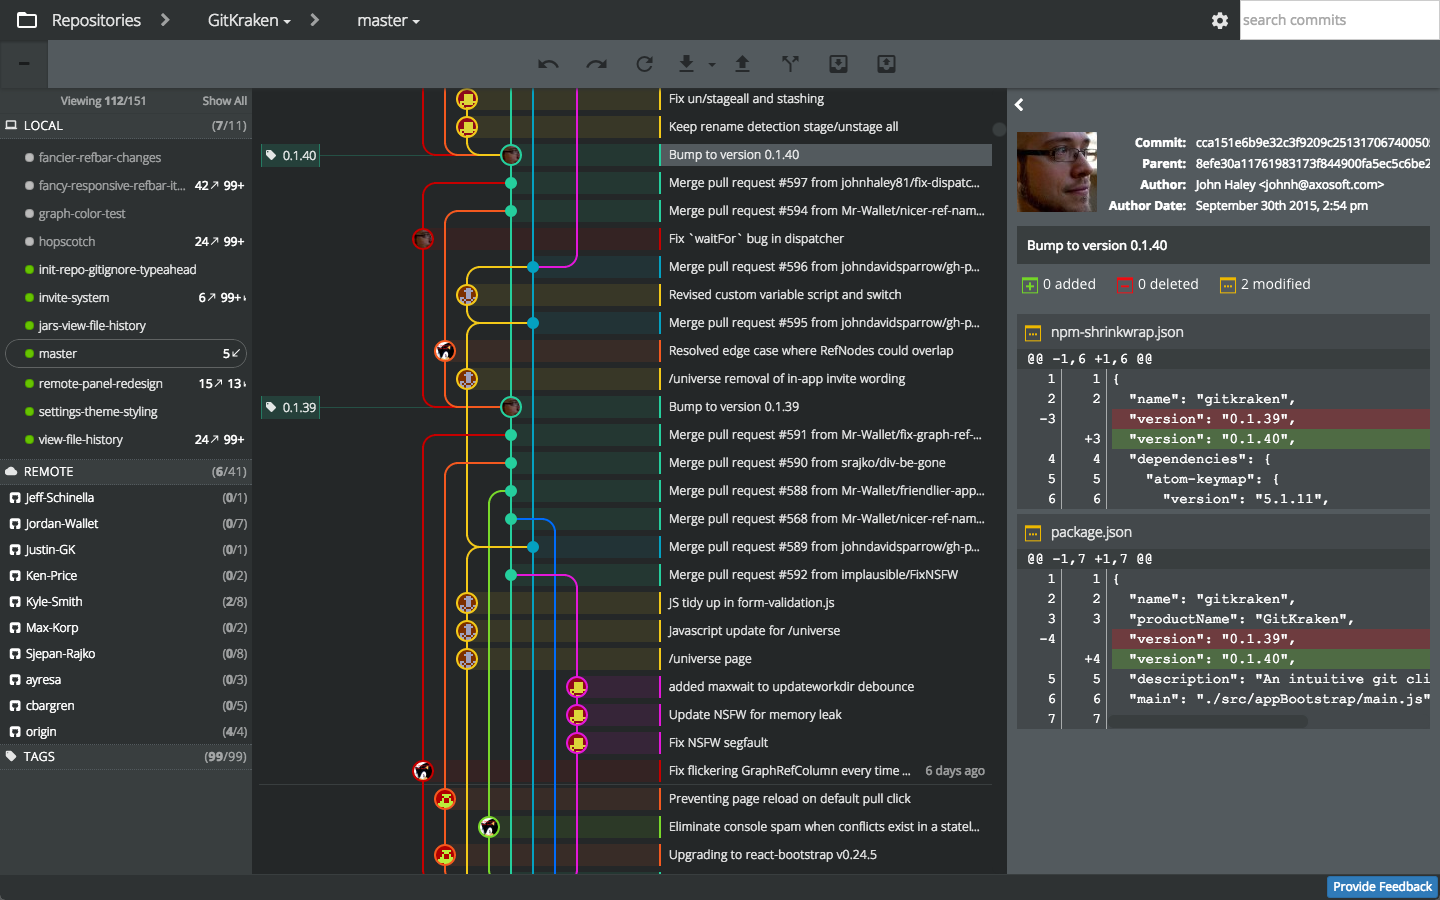
\includegraphics[width=0.8\linewidth]{Figures/introduction/gitkraken_main.png}
  \caption{Screenshot of the main view in GitKraken}
  \label{fig:gitkraken_main}
\end{figure}

GitLab and GitHub are both online repository hosts, with
visualization and summarization provided as well. While the GitLab
visualization does not appear to provide any additional information, the
visualization provided by GitHub takes advantage of additional internal
knowledge to display information about forks. Through this
visualization, GitHub displays the branch history of the repository
network, including the branches of the main repository and forks from
that. Giteye and most of the other visualizations are relatively
conventional, simply cleaning up the interface of Gitk, the visualizer
that is shipped with git. With the exception of Gitk, no GUI visualizers
are able to produce a visualization for the Linux repository, due to its
size. The GitHub visualizer displays an error message, stating that
there are too may forks to display. The GitKraken interface will freeze
and eventually crash while trying to load the repository, while Giteye
and the other visualizers will consume all of the system memory before
they are able to produce a visualization. The Gitk interface is the
least polished, but is able to produce a visualization of the
repository.

\begin{figure}[htpb]
  \centering
  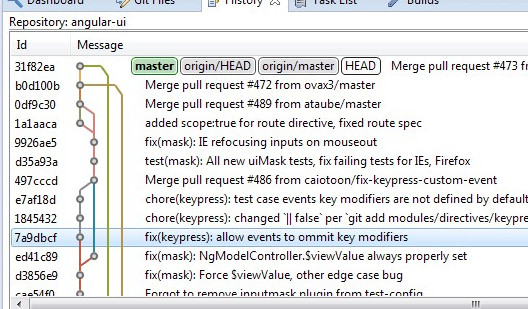
\includegraphics[width=0.8\linewidth]{Figures/introduction/giteye_graph.jpg}
  \caption{Screenshot of Giteye DAG view of a repository}
  \label{fig:giteye_screenshot}
\end{figure}

\begin{figure}[htpb]
  \centering
  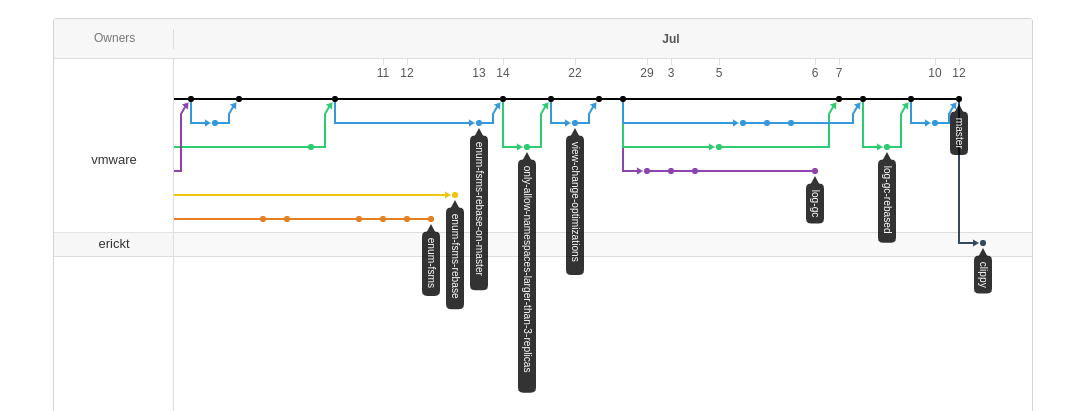
\includegraphics[width=0.8\linewidth]{Figures/introduction/github_dag.png}
  \caption{GitHub online network view of a repository}
  \label{fig:github_dag_screenshot}
\end{figure}

\begin{figure}[htpb]
  \centering
  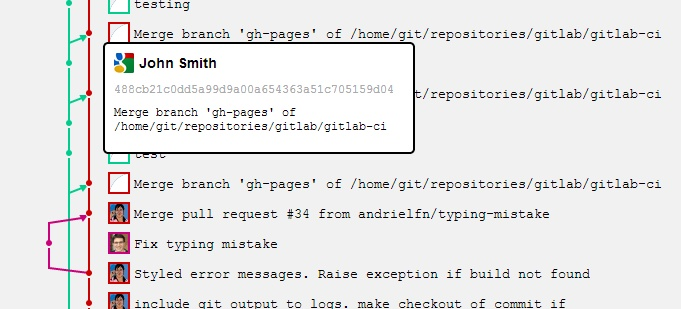
\includegraphics[width=0.8\linewidth]{Figures/introduction/gitlab_graph.jpg}
  \caption{GitLab online graph view}
  \label{fig:gitlab_dag_screenshot}
\end{figure}

\section{Thesis Organization}\label{sec:thesis_organization}

This \paper{} is organized as follows. Chapter~\ref{chap:background}
contains background information about the motivation, the Linux
repository, and the structure of git.

Chapter~\ref{chap:model} introduces the \mt{} model. This chapter
includes a description of the model, an algorithm to convert the from
the DAG to the \mt{}, and an evaluation of the resulting trees.

Chapter~\ref{chap:design_and_implementation} introduces \tool{},
providing the use-cases that were being targeted. This chapter also
includes the features that were implemented into \tool{}, including the
search engine, the summarization tables, and the tree visualizations.
More details on how the tool was implemented are included in
Chapter~\ref{chap:implementation_details}.

Chapter~\ref{chap:evaluation} includes the methodology and results of a
two-part study. The first part evaluates user comprehension of the DAG
and the second part compares visualizations and summarizations of the
DAG in Gitk against the visualizations and summarizations of the \mt{}
in \tool{}.

Chapter~\ref{chap:discussion} discusses the results of the study
providing more insight on the results. The chapter includes observations
from the study, and the comments from one of the members of the study
who had worked as a release manager, and a description and algorithm for
an updated \mt{} that takes into account the comments and observations
from the study. The chapter concludes with the limitations of the work
and the future work.

Chapter~\ref{chap:conclusion} concludes that paper, reiterating the
problem and how it was solved.
